\documentclass[12pt,a4paper,norsk]{article}
\usepackage[norsk]{babel}
\usepackage[utf8]{inputenc}

\usepackage{natbib}
\usepackage{graphicx}

\title{IT1901 \\ Prosjektrapport}
\author{Gruppe 08 \\ 
    755200, 741068, 757688,\\
    757676, 755591, 757787, \\
    757701, 757734, 757770}
\date{Oktober 2015}

\renewcommand{\contentsname}{Innhold}
\renewcommand\refname{Referanser}

\begin{document}
	\pagenumbering{gobble}
	\maketitle
	\newpage
	\pagenumbering{arabic}
	\tableofcontents
	\newpage
	\section{Introduksjon}

%For referanser skriv \cite{referansenavn}
%og om du vil oppgi sidetall \cite[Side 1-3]{referansenavn}

%%For å inkludere bilder i rapporten må du legge bildet i img-mappen og inkludere bildet på en slik måte:
%	\begin{figure}[h!]
%  		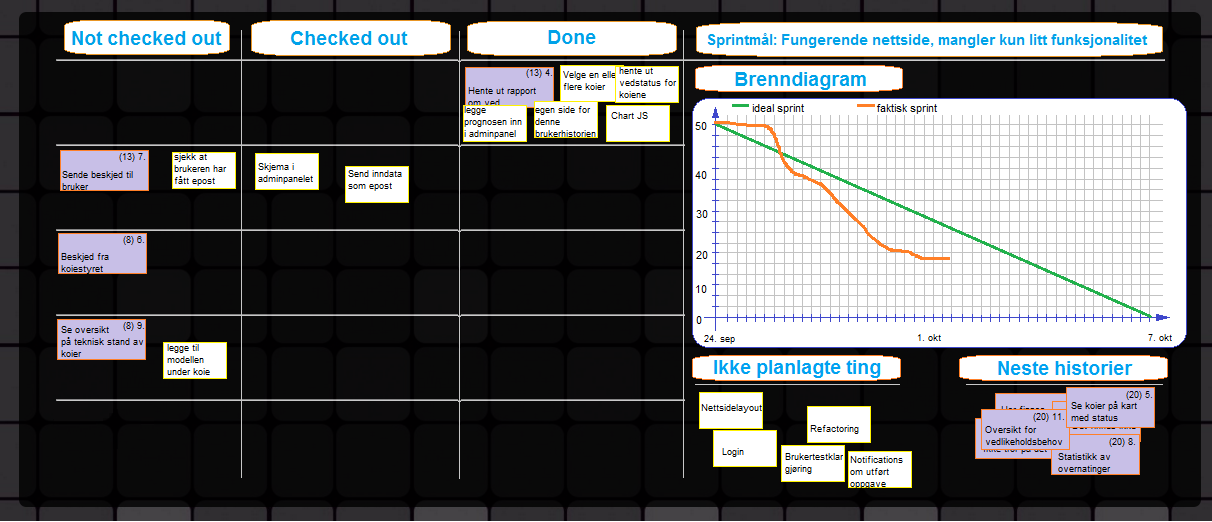
\includegraphics[width=\linewidth]{img/image00.png}
%  		\caption{Scrum Task-board, with burndown chart}
%  		\label{fig:task-board}
%	\end{figure}
%	Figur \ref{fig:task-board} viser...

Dette prosjektet er et gruppeprosjekt gitt i faget IT1901 - Informatikk prosjektarbeid 1, ved NTNU, høst 2015. Målet med prosjektet og faget er å gi deltagerne et innblikk hvordan det er å jobbe i større gruppeprosjekter og arbeidsmetoder hvor en tredjepart er med i prosessen. I dette prosjektets tilfelle er tredjeparten en kunde, som skal ta i bruk programmet. Prosjektet skal lære hvordan gruppeprosjekter gjennomføres og gi erfaringer rundt programmeringsverktøy, arbeidsmodeller og den smidige arbeidsmetoden Scrum.

\subsection{Problemstilling}

Gruppen skal utvikle et administrasjonssystem for NTNUI Koiene. Systemet skal være et tillegg til NTNUI Koiene sine allerede eksisterende websider, og gjøre det enklere å drifte koiene. Det skal for eksempel være mulig for brukere å rapportere vedstatus og ødelagte ting, samt få beskjed om å ta med seg ting til en reservert koie. Medlemmer av Koiestyret skal kunne se disse rapportene og bruke de til å planlegge veddugnader og reparasjoner.

Dette programmet skal gruppen utvikle etter kundens ønsker og behov, kunden har tildelt en rekke brukerhistorier som skal være oppfylt i det ferdige produktet.

	\section{Gruppen og rutiner}
	
\subsection{Rutiner og timeplan}

Det første gruppen måtte løse var timeplanen for prosjektet. Ettersom en studentarbeidsuke er på 40 timer, og vi har 4 fag i semesteret, bestemte vi som gruppe for å møtes og jobbe sammen 10 timer fordelt på 3 dager i uka.

\begin{itemize}
  \item[] Mandager fra 9:15 - 11:00 
  \item[] Torsdager fra 8:15 - 12:00
  \item[] Fredager fra 10:15 - 14:00
\end{itemize}

Dette fordi det gikk opp med de forskjellige timeplanene og gruppen var innstilt på at korte økter som dette ville holde produktiviteten på de timene oppe og konstruktive. 

\subsection{Gruppen og ansvarsfordeling}

Tidlig bestemte gruppen seg for at vi ville at alle skulle delta innom forskjellige arbeidsoppgaver, og ikke låses i for fastsatte roller. Dette fordi vi ville dele kompetansen så mye som mulig og la alle få litt erfaring i de forskjellige aspektene ved prosjektet. På den måten får man gjort seg mindre avhengig av enkeltpersoner, og får aktivisert gruppemedlemmer så mye som mulig. 

	\section{Arbeidsprosess}
	\subsection{Scrum i teori}
	\subsubsection{Produkt-backloggen}
	\subsubsection{Sprintplanleggingsmøtet}
	\subsubsection{Release-plan}
	\subsubsection{Daglig Scrum}
	\subsubsection{Retrospektiv-møtet}
	\subsubsection{Scrum-roller}
	\subsubsection{Task-board}
	\subsection{Scrum i praksis}
	\subsubsection{Sprint}
	\subsubsection{Brukerhistorier}
	\subsubsection{Task-board}
	\subsubsection{Retrospektiv}
	\subsubsection{Sprintgjennomgang}
	\section{Risikoanalyse}
	\section{Produkt}

\newpage
\addcontentsline{toc}{section}{Referanser}
\bibliographystyle{agsm}
\bibliography{referanser}

\end{document}

